\documentclass[11pt]{article}

\usepackage[T1]{fontenc}
\usepackage[utf8]{inputenc}
\usepackage[english]{babel}
\usepackage[margin=1in]{geometry}
\usepackage{lmodern}
\usepackage{microtype}
\usepackage{mathtools}
\usepackage{amssymb}
\usepackage{amsthm}
\usepackage{graphicx}
\usepackage{booktabs}
\usepackage{array}
\usepackage{caption}
\usepackage{enumitem}
\usepackage{fancyhdr}
\usepackage{makecell}
\usepackage[numbers,sort&compress]{natbib}
\usepackage{orcidlink}
\usepackage{tabularx}
\usepackage{titling}
\usepackage{xurl}
\usepackage{hyperref}
\usepackage{tikz}
\usetikzlibrary{arrows.meta, positioning, fit}
\title{To XOR a Stone with Six Birds: Closure Diagnostics for Emergent Bits, Gates, and Booleanity}
\author{Ioannis Tsiokos\,\orcidlink{0009-0009-7659-5964}}
\date{March 9, 2026}
\hypersetup{
  pdftitle={To XOR a Stone with Six Birds: Closure Diagnostics for Emergent Bits, Gates, and Booleanity},
  pdfauthor={Author names withheld for review},
  hidelinks
}
\urlstyle{same}
\captionsetup{
  font=small,
  labelfont=bf,
  labelsep=period
}
\captionsetup[table]{skip=6pt}
\captionsetup[figure]{skip=6pt}
\setlist[enumerate]{leftmargin=*, itemsep=2pt, topsep=4pt}
\setlength{\droptitle}{-3.2em}
\pretitle{\begin{center}\LARGE\bfseries}
\posttitle{\par\end{center}\vspace{0.5em}}
\preauthor{\begin{center}\normalsize}
\postauthor{\par\end{center}\vspace{-0.4em}}
\predate{\begin{center}\small}
\postdate{\par\end{center}\vspace{0.6em}}
\setlength{\emergencystretch}{2em}
\clubpenalty=10000
\widowpenalty=10000
\displaywidowpenalty=10000
\interfootnotelinepenalty=10000
\allowdisplaybreaks[2]
\theoremstyle{definition}
\newtheorem{definition}{Definition}
\newcommand{\num}[2][]{#2}
\setlength{\bibsep}{2pt plus 0.3ex}
\fancypagestyle{firstpage}{%
  \fancyhf{}
  \fancyfoot[C]{\scriptsize Automorph Inc., Wilmington, DE, USA \quad \texttt{ioannis@automorph.io} \quad \mbox{DOI: \href{https://doi.org/10.5281/zenodo.18919370}{10.5281/zenodo.18919370}} \quad \textcopyright\ 2026 \quad CC-BY 4.0 \quad Preprint --- not peer reviewed.}
  \renewcommand{\headrulewidth}{0pt}
  \renewcommand{\footrulewidth}{0pt}
}

\begin{document}

\maketitle
\thispagestyle{firstpage}

\begin{abstract}
Boolean logic is usually treated as a formal starting point. We ask instead when a substrate actually earns a logic layer. In the Six Birds emergence calculus---P1 operator rewrite, P2 gating/constraints, P3 protocol holonomy, P4 sectors/invariants, P5 packaging, and P6 accounting/audit---we define a logic layer as an audited closure of packaged predicates under induced dynamics. This yields two complementary views. In the feasibility view, propositions are definable feasible sets and connectives are their stable closure operations. In the operator view, bits are packaged equivalence classes and gates are macro-updates induced by the underlying dynamics. We implement quantitative diagnostics for both views: metastability, route mismatch, closure defect, gate error, conditional entropy, unretained input information, and entropy-production audits. Across controlled finite Markov laboratories we obtain four main results. First, parity/XOR-type variables are unusually robust coarse variables: the parity lens beats the median random binary partition across the full tested grid. Second, NOT, AND, and reversible XOR embeddings exhibit distinct closure regimes under noise, staging, and timescale stress. Third, when a reversible CNOT embedding is coarse-grained to an erased XOR output, closure degrades sharply and unretained input information increases by more than eightfold relative to the retained view. Fourth, a minimal unsupervised discovery pipeline recovers stable bits and reconstructs a NOT gate directly from transition structure. The result is a falsifiable criterion for when a system has logic at a layer---and for which logic it has---without treating logic as fundamental.
\end{abstract}

\noindent\textbf{Keywords:} emergent logic; coarse-graining; closure diagnostics; parity and XOR; reversible computation; information loss.

\medskip

\noindent\textbf{Contribution summary.} This paper contributes a layer-relative definition of logic as audited closure, an operational diagnostic suite for detecting bits and gates in coarse-grained dynamics, and controlled demonstrations of parity robustness, reversible-versus-erased gate divergence, and unsupervised recovery of packaged bits and a NOT gate from transition structure.


\section{Introduction}
\label{sec:introduction}

Many canonical discussions of physical computation and reversible logic begin from a prior vocabulary of bits, registers, and truth tables \cite{landauer1961,bennett1973,fredkintoffoli1982conservative,bennett1982thermodynamics}. That question is important, but it already assumes the existence of a symbolic layer. Before implementation lies a harder prior question: when does a coarse-grained layer deserve to be described in logical terms at all? A system may admit labels that look like \(0\) and \(1\) without supporting stable predicates, reliable negation, or closed gate operators. In that case, logic has been projected onto the system rather than discovered in it.

This paper gives an operational answer. We work in the Six Birds emergence calculus \cite{tsiokos2026sixbirds}, whose six primitives are P1 operator rewrite, P2 gating / constraints, P3 autonomous protocol holonomy, P4 sectors / invariants, P5 packaging, and P6 accounting / audit. Our central claim is that logic is not a seventh primitive and not a hidden Platonic layer. It is a layer-relative achievement of these six ingredients. A system has a logic layer when packaged binary predicates become stable, when induced macro-operators close on those predicates, and when the reliability and loss of that closure can be audited. In one sentence: a logic layer is an audited closure of packaged predicates under induced dynamics.

That perspective shifts the usual starting point. In the feasibility view, propositions are not abstract atoms but definable feasible sets, and logical connectives are stable closure operations on those sets. In the operator view, bits are not fundamental carriers but packaged equivalence classes of microstates, and gates are macro-updates induced by the underlying dynamics. The two views are complementary. The first gives semantics to truth; the second tells us when those semantics are executable by a substrate. Together they replace the familiar question ``how is logic implemented?'' with the more basic question ``when has logic emerged strongly enough to close?'' \cite{pawlak1982rough,ellerman2010partitions,shalizi2025macrostate}

The title emphasizes XOR for a reason. Parity-like variables aligned with a system's invariant or sector structure are often especially natural coarse variables; in this paper parity is the controlled test case for that more general idea \cite{simonando1961aggregation,shalizi2025macrostate,barnettseth2023dynamical}. It survives cancellation of micro-detail, aligns naturally with invariant structure, and persists under coarse-graining in regimes where more brittle variables do not. That does not make XOR metaphysically privileged. It makes parity an empirical test case for the broader thesis of the paper: some logical forms are easier for substrates to stabilize than others. The right question is therefore not whether a substrate can be made to emulate a desired truth table in principle, but which logical distinctions it supports natively, robustly, and at what accounting cost.

Our emphasis is therefore diagnostic rather than merely implementational. We introduce a suite of quantitative tests for candidate logic layers: predicate stability, route mismatch, closure defect, gate error, conditional entropy, unretained input information, and entropy-production audits. These tests distinguish genuine closure from symbolic overinterpretation. They let us ask whether two routes to the same purported macro-description agree, whether a packaged bit persists long enough to matter, whether a gate is really a closed macro-operator rather than a protocol artifact, and whether information that appears to disappear has in fact been erased, hidden, or retained in side variables. This is also where the Six Birds grammar becomes empirically useful: packaging makes predicates possible, constraints give them meaning, protocol effects create route dependence, sectors stabilize them, rewrite repairs or redesigns closure, and accounting determines what can be maintained without cheating.

Our starting point is therefore closer to coarse-graining and audited closure than to implementation-first accounts of logic. Internally, the paper draws on the Six Birds foundations \cite{tsiokos2026sixbirds} and on the broader closure-and-substrate program developed in \cite{tsiokos2026countstone,tsiokos2026minsubstrate}. Externally, the descent of dynamics to coarse variables is related to lumpability and effective Markov aggregation \cite{kemeny1976finite,buchholz1994lumpability,simonando1961aggregation,givon2004extracting}, while the distinction between retained and erased descriptions connects directly to the classic literature on irreversibility and reversible computation \cite{landauer1961,bennett1973,bennett1982thermodynamics}.

The payoff is a controlled program rather than a metaphor. We build finite Markov laboratories in which NOT, AND, and reversible XOR embeddings can be realized with tunable noise, metastability, and coarse-graining. Within those laboratories we ask four concrete questions. First, which binary coarse variables close most robustly under the induced dynamics? Second, how do familiar gates behave as noise, staging barriers, and timescale stress are varied? Third, what changes when a reversible embedding is coarse-grained to an apparently simpler but information-losing gate? Fourth, can stable bits and gates be recovered from transition structure without declaring them by hand in advance?

This paper answers all four. Parity beats the median random binary partition across the full tested grid, making XOR the paper's clearest instance of a substrate-native logical distinction. NOT, AND, and reversible XOR embeddings exhibit distinct closure regimes rather than a single uniform notion of Boolean success. When a reversible CNOT embedding is viewed through an erased XOR output, closure degrades sharply and unretained input information increases by more than an order-one factor, showing that reversible embedding and erased output are not the same logical object. Finally, a minimal discovery pipeline recovers stable packaged bits and reconstructs a NOT gate directly from transition structure, showing that the framework can find logic rather than merely redescribe it.

\paragraph{Contributions.}
This paper makes three contributions. First, it gives a layer-relative definition of logic in the Six Birds framework: a logic layer is an audited closure of packaged predicates under induced dynamics. Second, it introduces operational diagnostics that distinguish genuine logic layers from projected symbolic descriptions. Third, it demonstrates the framework in controlled finite laboratories, yielding a parity-robustness result, a reversible-versus-erased gate separation, and an unsupervised recovery result for both packaged bits and a NOT gate.

The paper is not a general survey of physical computation, nor a claim that Boolean logic is the only endpoint of coarse-graining. On the contrary, the viewpoint developed here is pluralistic: the logic a layer ``has'' depends on which closures it can stably support. In particular, complement, negation, and even the availability of binary truth carriers are empirical achievements rather than automatic givens. What we do show is that once closure, packaging, and audit are treated as first-class objects, logic becomes something a substrate can earn, lose, or support only partially.

The remainder of the paper develops this claim in stages. Section~\ref{sec:framework} formalizes the notion of a logic layer through packaging, definability, and induced closure. Section~\ref{sec:diagnostics-methods} introduces the diagnostics and the controlled finite laboratories used throughout. Section~\ref{sec:results-parity} shows that parity is an unusually robust coarse variable. Section~\ref{sec:results-phase} studies gate closure regimes for NOT, CNOT, and AND across noise, staging, and timescale stress. Section~\ref{sec:results-reversible} compares reversible embedding to erased XOR and quantifies the resulting accounting differences. Section~\ref{sec:results-discovery} shows that bits and a NOT gate can be recovered directly from transition structure. Section~\ref{sec:discussion} closes by returning to the broader question of what it means for a layer to have a logic at all.

\section{Logic Layers, Packaging, and Closure}
\label{sec:framework}

We do not rederive the full Six Birds formalism here. For the present paper only the pieces needed to speak about logic are essential: a lens that fixes what is observable, a packaging step that stabilizes those observables into reusable carriers, an induced dynamics that may or may not close on the packaged variables, and an audit that measures persistence, mismatch, and loss. In Six Birds terms, P5 supplies the package, P2 supplies feasibility semantics, P4 supplies metastability or sector structure, P1 governs whether new effective operators can be introduced, P3 diagnoses route dependence, and P6 keeps the accounting honest. This section isolates those ingredients and turns them into a concrete criterion for what we will call a \emph{logic layer} \cite{tsiokos2026sixbirds}.

\subsection{Lenses, definability, and packaged predicates}

Let \(Z\) denote the microstate space and let
\[
f: Z \to X
\]
be a lens or coarse-graining map into a smaller label space \(X\). The fibers of \(f\) specify which microstates the candidate layer refuses to distinguish. A binary predicate \(h: Z \to \{0,1\}\) is \emph{definable} at that lens when it is constant on fibers, equivalently when there exists a macro-predicate \(\tilde h : X \to \{0,1\}\) such that
\[
h = \tilde h \circ f.
\]
We write \(\Sigma_f\) for the family of events or predicates definable from \(f\). \(\Sigma_f\) is the expressive content of the layer: if a distinction is not definable there, then it is not available as a logical statement at that layer.

Packaging is the step that turns a mere definable distinction into a reusable symbol carrier. In the binary case, a package is a map
\[
\Pi : Z \to \{0,1\},
\]
with many microstates assigned to the same label because they are treated as equivalent for the purposes of the layer. For a definable event \(A \in \Sigma_f\), the associated packaged predicate is simply the indicator
\[
\Pi_A(z) = \mathbf{1}[z \in A].
\]
This is the point at which P5 becomes indispensable: truth values are not primitive objects but compressed labels of microstates. They remain meaningful only when P4 supplies enough staging, metastability, or sector structure for those labels to persist across the timescale on which the layer is supposed to operate.

\subsection{Two complementary views of logic}

The first view is semantic. In the \emph{feasibility view}, propositions are definable feasible sets and logical connectives are stable closure operations on those sets. Once a universe of admissible states is fixed, the familiar connectives are forced:
\[
A \wedge B = A \cap B,\qquad
A \vee B = A \cup B,\qquad
\neg A = Z \setminus A,
\]
and, for parity,
\[
A \oplus B = (A \setminus B) \cup (B \setminus A).
\]
On this view, logic is not an extra ontology layered on top of physics. It is the algebra of feasible distinctions that a lens can express and a substrate can stabilize. P2 appears here as the semantics of admissibility: propositions are gates on what states are allowed, and contradictions are simply empty feasible sets.

The second view is operational. In the \emph{operator view}, a packaged bit matters only if the substrate supports induced updates on it. Let \(F : Z \to Z\) denote a micro-update, or more generally let \(P\) be a Markov kernel on \(Z\). A macro-operator \(g\) is induced on a package \(\Pi\) when the packaged description closes, at least approximately, under the underlying dynamics:
\[
\Pi(F(z)) \approx g(\Pi(z)).
\]
At the level of distributions, if \(Q_f\) denotes pushforward through the lens and \(U_f\) denotes a canonical lift back to packaged microdescriptions, the associated empirical endomap is
\[
E_{\tau,f}(\mu) = U_f\!\bigl(Q_f(\mu P^\tau)\bigr).
\]
This is the reduce--evolve--repackage route.
In finite-state language, the same descent problem is the one studied by lumpability theory for Markov chains \cite{buchholz1994lumpability}.
A genuine macro law requires it to agree, up to a controlled defect, with the route that reasons directly at the packaged level. P1 enters here because effective operators sometimes need to be rewritten or promoted to close cleanly. P3 enters here because route mismatch is precisely the sign that ordering, hidden protocol state, or evaluation schedule is still leaking through the coarse description.

The two views are inseparable in practice. Feasibility without operator closure gives semantics that cannot be executed. Operator closure without feasibility semantics gives a convenient signal-processing description but not yet a logic. A logic layer appears only when the same packaged distinctions support both views at once.

\begin{definition}[Logic layer]
\label{def:logic-layer}
Fix a microstate space \(Z\), a lens \(f : Z \to X\), and an evaluation window \(\tau\). A \emph{logic layer} at \((f,\tau)\) consists of a nontrivial family \(\mathcal{B} \subseteq \Sigma_f\) of binary packaged predicates together with induced macro-updates such that:
\begin{enumerate}
    \item \textbf{Stability.} Each \(b \in \mathcal{B}\) is metastable on the timescale \(\tau\).
    \item \textbf{Closure.} The relevant micro-updates descend to macro-operators on the packaged variables with small closure defect.
    \item \textbf{Feasibility semantics.} Each \(b \in \mathcal{B}\) is the indicator of a stable feasible set, and the connective operations required at the layer remain definable there.
    \item \textbf{Auditability.} Persistence, route agreement, and information loss are measurable by explicit diagnostics.
\end{enumerate}
When these conditions fail, a symbolic description may still be convenient, but it does not constitute a closed logic layer in the sense used in this paper.
\end{definition}

Figure~\ref{fig:logic-layer-overview} summarizes the architecture of the notion introduced in Definition~\ref{def:logic-layer}: microstates enter the candidate logic layer only through packaging, and the resulting predicates count as logical only when both their feasibility semantics and their induced operators survive explicit audit.

\begin{figure}[t]
    \centering
    \resizebox{0.94\linewidth}{!}{\begin{tikzpicture}[
    >=Latex,
    font=\small,
    line width=0.5pt,
    box/.style={
        draw,
        rounded corners,
        fill=black!2,
        align=left,
        inner sep=6pt,
        text width=#1
    },
    box/.default=3.3cm,
    arrowlabel/.style={
        font=\footnotesize,
        align=center,
        fill=white,
        inner sep=1pt
    },
    note/.style={
        font=\footnotesize\itshape,
        align=center,
        fill=white,
        inner sep=1pt
    }
]

\node[box=2.9cm] (micro) {
\textbf{Microstates \(Z\)}\\[2pt]
\(\bullet\ z_1 \qquad \bullet\ z_4\)\\
\(\bullet\ z_2 \qquad \bullet\ z_5\)\\
\(\bullet\ z_3 \qquad \bullet\ z_6\)\\[2pt]
messy substrate detail
};

\node[box=3.5cm, right=16mm of micro] (packaged) {
\textbf{P5 packaged predicates / bits}\\[2pt]
\(h=\tilde h \circ f\)\\
\(\Pi_A(z)=\mathbf{1}[z\in A]\)\\[2pt]
\(\boxed{0}\ \ \boxed{1}\) stable carriers
};

\node[note, above=2mm of packaged] (p4note) {P4 staging / sectors\\keep carriers stable};

\node[box=3.4cm, right=18mm of packaged] (audit) {
\textbf{P6 audit / closure checks}\\[2pt]
stability \(S_\tau\)\\
route mismatch RM\\
defect \(\Delta_{\tau,f}\)\\
loss \(U_{\text{loss}}\)\\
apparent EPR \(\sigma_{\mathrm{app}}\)
};

\node[box=3.9cm, above=9mm of audit] (feasibility) {
\textbf{P2 feasibility semantics}\\[2pt]
\(A\wedge B=A\cap B\)\\
\(A\vee B=A\cup B\)\\
\(\neg A=Z\setminus A\)\\
\(A\oplus B=A\triangle B\)
};

\node[box=3.9cm, below=9mm of audit] (operators) {
\textbf{P1 induced operators}\\[2pt]
\(\Pi(F(z)) \approx g(\Pi(z))\)\\
\(E_{\tau,f}(\mu)=U_f(Q_f(\mu P^\tau))\)
};

\node[note, below left=2mm and -5mm of feasibility.south east, anchor=north west] (p3note) {P3 route agreement\\must be checked};

\draw[->, thick] (micro.east) -- node[arrowlabel, above]{lens \(f\)} (packaged.west);
\draw[->, thick] (packaged.north east) -- (feasibility.west);
\draw[->, thick] (packaged.south east) -- (operators.west);
\draw[->, thick] (feasibility.south) -- (audit.north);
\draw[->, thick] (operators.north) -- (audit.south);

\node[draw=black!50, dashed, rounded corners, inner sep=8pt, fit=(packaged)(p4note)(feasibility)(operators)(audit)(p3note)] (layer) {};
\node[font=\small\bfseries, above=1mm of layer] {Logic layer at \((f,\tau)\)};

\end{tikzpicture}
}
    \caption{A logic layer is an audited closure of packaged predicates. A lens \(f\) and a packaging map compress microstates into stable binary carriers. Those carriers support two complementary views at once: feasibility semantics on definable sets and induced macro-operators on packaged symbols. The layer counts as logical only when the resulting closure survives explicit audit through stability, route mismatch, closure defect, and unretained input information diagnostics.}
    \label{fig:logic-layer-overview}
\end{figure}

\subsection{Why the criterion is layer-relative}

Definition~\ref{def:logic-layer} is intentionally stricter than merely being able to label states by zero and one. A candidate bit must remain stable long enough to matter, must support a descended operator calculus, and must survive audit. This is why the six primitives are complementary rather than redundant. P5 packages the carrier; P4 keeps it from dissolving immediately; P2 makes it semantically meaningful; P1 determines whether an effective operator vocabulary can be stabilized; P3 detects route dependence and protocol residue; P6 determines what must be paid to maintain the whole arrangement.

The criterion is also intentionally broader than classical Booleanity. Complement and negation appear naturally when the relevant complements remain definable and stable at the lens. But nothing in Definition~\ref{def:logic-layer} forces every layer to have those complements available at low cost. For that reason we speak of a \emph{logic layer} rather than a \emph{Boolean layer}. The finite laboratories studied in this paper are classical-looking enough to realize NOT, AND, and XOR cleanly, but the framework itself is meant to diagnose which closures a layer actually supports rather than to decree them in advance.

This perspective clarifies what the rest of the paper will measure. Section~\ref{sec:diagnostics-methods} turns the four clauses of Definition~\ref{def:logic-layer} into concrete observables: predicate stability measures the first clause, route mismatch and closure defect probe the second, feasible-set and gate semantics ground the third, and unretained input information and entropy-production proxies support the fourth. The results sections then use those diagnostics to show that parity is unusually robust as a packaged distinction, that familiar gates occupy different closure regimes, and that reversible embedding and erased output are distinct logical objects rather than notational variants.

\section{Diagnostics and Methods}
\label{sec:diagnostics-methods}

Definition~\ref{def:logic-layer} gives four requirements for a logic layer: stability, closure, feasibility semantics, and auditability. This section turns those four requirements into measurable quantities and summarizes the controlled laboratories in which they are evaluated. The important methodological point is that the paper is not reporting live computations from the manuscript source. All numerical values reported in Sections~\ref{sec:results-parity}--\ref{sec:results-discovery} are taken from the frozen result bundle under \path{results/final_claims/} and the source artifacts it summarizes. The manuscript does not recompute those values during drafting; it only defines the diagnostics and interprets the frozen outputs.
Methodologically, this follows the broader Six Birds insistence that closure claims be paired with explicit audit rather than inferred from symbolic convenience alone \cite{tsiokos2026countstone,tsiokos2026minsubstrate}.

\subsection{Stability and closure diagnostics}

The first diagnostic is \emph{predicate stability}. For a binary packaged predicate \(b : Z \to \{0,1\}\), a Markov kernel \(P\) on \(Z\), an evaluation horizon \(\tau\), and an initial micro-distribution \(\mu\), we measure
\[
S_\tau(b;\mu)
=
\sum_{i,j} \mu_i (P^\tau)_{ij}\,\mathbf{1}[b(i)=b(j)].
\]
Large \(S_\tau\) means that the packaged distinction survives the timescale on which the layer is supposed to operate. In the experiments below, this quantity is used both for stable input bits in the gate laboratories and for candidate partitions in the discovery pipeline.

The second diagnostic is \emph{route mismatch} (RM), which asks whether states placed in the same coarse cell really have the same coarse transition behavior. For a lens \(f : Z \to X\), define the coarse transition profile of a microstate \(i\) by
\[
R_\tau^f(i,x)
=
\sum_{j : f(j)=x} (P^\tau)_{ij}.
\]
If \(B_x=f^{-1}(x)\) is the fiber of \(x\) and \(\bar\omega_i^{(x)}\) are normalized weights within that fiber, then the induced macro row is
\[
K_{\tau,f}(x,\cdot)
=
\sum_{i\in B_x} \bar\omega_i^{(x)} R_\tau^f(i,\cdot),
\]
and the route mismatch is the weighted within-fiber discrepancy
\[
\mathrm{RM}_\tau(f)
=
\sum_x \sum_{i\in B_x}
\bar\omega_i^{(x)}
\bigl\|
R_\tau^f(i,\cdot)-K_{\tau,f}(x,\cdot)
\bigr\|_1.
\]
RM vanishes when coarse-grained transition behavior is fiberwise consistent. It grows when the lens collapses states whose macro futures differ. In the parity experiment we compare RM across parity, AND, and random binary lenses; in the phase-diagram and reversible-versus-erased experiments we also use stationary weighting to prevent rare states from dominating the metric.

A third closure diagnostic compares two different reduction routes. Given pushforward \(Q_f\) through the lens and a canonical lift \(U_f\) back to a packaged microdescription, the \emph{closure defect}, implemented here as a distribution commutation defect, is
\[
\Delta_{\tau,f}(\mu)
=
\left\|
Q_f(\mu P^\tau)
-
Q_f\!\bigl(U_f(Q_f(\mu))P^\tau\bigr)
\right\|_1.
\]
The first term evolves microscopically and then reduces; the second reduces, repackages, evolves, and reduces again. Small defect means that the packaged description is genuinely closed under the dynamics. Large defect indicates that hidden microstructure or protocol residue is still leaking through the purported logic layer.

Taken together, \(S_\tau\), RM, and \(\Delta_{\tau,f}\) operationalize the first two clauses of Definition~\ref{def:logic-layer}. Stability measures persistence. RM and closure defect measure whether closure has actually been achieved rather than merely asserted.

\subsection{Gate-channel and information diagnostics}

For gate-like behavior we work with induced input--output channels. Let \(f_{\mathrm{in}}\) be a current-state input labeling and \(f_{\mathrm{out}}\) a future-state output labeling. For each input label \(u\), we initialize uniformly over the microstates satisfying \(f_{\mathrm{in}}=u\), evolve for \(\tau\) steps, and read the output label \(y\). This defines a channel
\[
C_\tau(y\mid u).
\]
All gate metrics in the paper are derived from this induced channel, using a uniform prior over input patterns unless explicitly noted otherwise.

If \(t(u)\) denotes the intended truth-table output for input \(u\), then the \emph{truth error} is
\[
\mathrm{err}_{\mathrm{truth}}
=
\frac{1}{|U|}
\sum_{u\in U}
\bigl[1 - C_\tau(t(u)\mid u)\bigr].
\]
This compares the induced channel to a chosen logical target. To measure how deterministic the channel is even without an externally supplied truth table, we also use the \emph{induced error}
\[
\mathrm{err}_{\mathrm{induced}}
=
\frac{1}{|U|}
\sum_{u\in U}
\left(1-\max_{y} C_\tau(y\mid u)\right),
\]
which vanishes only when the best-fit deterministic output is certain for every input class.

The corresponding uncertainty measure is the conditional entropy
\[
H(\mathrm{out}\mid \mathrm{in})
=
-
\frac{1}{|U|}
\sum_{u\in U}\sum_y
C_\tau(y\mid u)\log_2 C_\tau(y\mid u),
\]
with the usual convention that \(0\log 0 = 0\). This is the main entropy quantity reported in the phase-diagram results. It tracks the same phenomenon as induced error, but without collapsing uncertainty to an argmax summary.

For the accounting comparisons we also use standard channel-information quantities. With the same uniform input prior,
\[
I(\mathrm{in};\mathrm{out})
=
H(\mathrm{out}) - H(\mathrm{out}\mid \mathrm{in}),
\]
and we define the \emph{unretained input information} by
\[
U_{\text{loss}}
=
H(\mathrm{in}) - I(\mathrm{in};\mathrm{out}).
\]
This is the primary information-loss proxy in the reversible-versus-erased analysis. It measures how much input information is not recoverable from the reported output channel. We also track the simpler entropy-drop proxy
\[
\Delta H = H(\mathrm{in}) - H(\mathrm{out}),
\]
but the main comparison later in the paper is expressed in terms of \(U_{\text{loss}}\), because reversible embeddings can preserve output entropy while still hiding or discarding part of the input description.
The reversible-versus-erased comparison in Section~\ref{sec:results-reversible} is framed in the spirit of Landauer's analysis of irreversibility and Bennett's reversible-computation program \cite{landauer1961,bennett1973}.

Finally, to connect information processing with embodiment, we compute entropy-production rates. For a stationary distribution \(\pi\) of the micro-kernel \(P\), the micro-level entropy production rate is
\[
\sigma(P)
=
\sum_{i,j}
\pi_i P_{ij}
\log
\frac{\pi_i P_{ij}}{\pi_j P_{ji}},
\]
measured in nats per step. The corresponding \emph{apparent} coarse-grained entropy production is obtained by inducing a macro-kernel \(K_{\tau,f}\) on a lens \(f\) and then evaluating the same expression on that macro-kernel:
\[
\sigma_{\mathrm{app}}(f,\tau)
=
\sigma(K_{\tau,f}).
\]
Micro and apparent EPR coincide on the identity lens and can diverge under coarse-graining. In this paper they serve as audit variables rather than as stand-alone thermodynamic claims. All Shannon quantities are reported in bits; all entropy-production quantities are reported in nats per step.

\subsection{Finite logic laboratories}

The experiments are carried out in finite Markov laboratories built from a macro-register space \(X\) together with a micro-degeneracy factor \(d\), so that
\[
Z = X \times \{1,\dots,d\}.
\]
A single tick of the dynamics first applies a deterministic macro-update, then injects controlled output noise, then applies memory flips to designated stable bits, and finally redistributes probability uniformly across the \(d\) microstates of the destination macrostate. This last step enforces rapid within-fiber mixing and makes packaging explicit rather than implicit.

Three gate laboratories are used throughout. The NOT laboratory carries registers \((a,c)\), where \(a\) is a stable input bit and the gate sets \(c' = 1-a\). The AND laboratory carries \((a,b,c)\), where \(a\) and \(b\) are stable input bits and the gate sets \(c' = a \wedge b\). The reversible XOR embedding is implemented as a CNOT laboratory with registers \((a,b)\), where \(a\) is the stable control and the target updates as \(b' = a \oplus b\). Output noise is controlled by \(p_{\mathrm{gate}}\). Stable-input corruption is controlled either directly by \(p_{\mathrm{mem}}\) or indirectly through a barrier parameter via
\[
p_{\mathrm{mem}} = \text{base\_mem\_noise}\,e^{-\text{barrier}}.
\]
The phase-diagram sweeps vary \(p_{\mathrm{gate}}\), barrier, and \(\tau\). For CNOT, the \(\tau>1\) cases are interpreted as closure stress tests rather than as repeated evaluation of a single-step static truth table.

A fourth laboratory, the parity-sector model, is not a gate laboratory in the same sense. It is a two-bit system \((a,b)\) with controlled leakage between the even-parity and odd-parity sectors. Its purpose is to ask which binary coarse variables remain robust as noise and timescale vary. This is the laboratory used for the parity-versus-random-lens comparison.

\subsection{Discovery pipeline}

The final part of the methods asks whether stable bits and gates can be recovered from transition structure without declaring them by hand. For input-bit discovery we compute the second eigenvector of a reversibilized, symmetrized \(\tau\)-step operator and sweep threshold cuts through that vector to generate binary partitions. Each candidate partition is scored by metastability minus RM, so the preferred candidate is both persistent and closure-friendly. In the NOT and parity laboratories, the best-scoring recovered partitions agree with the intended packaged bits at the level reported later in Section~\ref{sec:results-discovery}.

Output-bit discovery is treated separately in the NOT gate reconstruction. There we first build bidirectional behavioral classes from outgoing rows and incoming columns of the kernel, enumerate binary partitions of those classes, and rank the candidates by future information gain over present redundancy. Intuitively, a good output partition should be informative about future behavior while not simply restating the current input partition. Once input and output partitions are selected, we form a balanced transition sample, infer the best-fit one-input gate, and record its error and conditional entropy. The recovered NOT result reported later in the paper is frozen in \path{results/final_claims/table_gate_discovery.csv} and the underlying source artifacts listed in the claim ledger.

The net effect of this methodology is that every clause of Definition~\ref{def:logic-layer} is tied to an explicit measurement. Stability is probed by \(S_\tau\), closure by RM and closure defect, gate semantics by channel error and entropy, and embodiment by unretained input information and entropy-production audits. The remaining sections simply read those diagnostics off the frozen result bundle for four different empirical questions: which coarse variables are robust, which gates close under stress, what changes under erasure, and whether bits and gates can be discovered rather than imposed.

\section{Parity Robustness}
\label{sec:results-parity}

Figure~\ref{fig:parity-robustness} is the empirical anchor for the title claim of the paper. The parity-sector laboratory is designed around controlled leakage between the even- and odd-parity sectors of a two-bit system, so the natural candidate coarse variable is the parity bit \(a \oplus b\). We compare that lens against two alternatives defined on the same underlying four macrostates: the familiar Boolean predicate \(a \wedge b\), and the median of a family of balanced random binary partitions. The comparison is intentionally closure-based rather than purely predictive. The plotted quantity is route mismatch (RM), so smaller values mean that the proposed binary variable is better aligned with the induced coarse dynamics.

\begin{figure}[t]
    \centering
    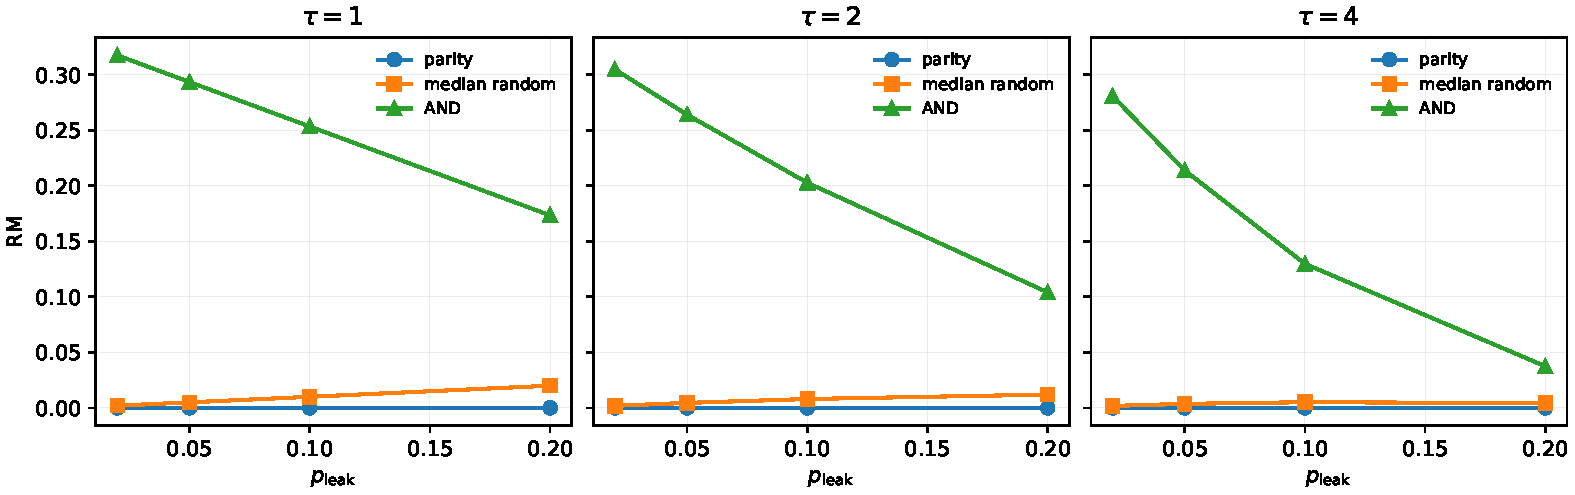
\includegraphics[width=\linewidth]{figures/parity_robustness.pdf}
    \caption{Route mismatch in the parity-sector laboratory for three candidate binary coarse variables: the parity lens \(a \oplus b\), the AND lens \(a \wedge b\), and the median balanced random binary partition. Each panel fixes \(\tau\) and scans leakage \(p_{\mathrm{leak}}\). Across the full tested grid, the parity lens remains essentially closure-aligned while the AND and median-random alternatives show systematically larger mismatch. The figure is rendered directly from \protect\path{results/final_claims/figure_parity_robustness.csv}.}
    \label{fig:parity-robustness}
\end{figure}

The main result is absolute across the tested grid. In the frozen bundle, the parity lens beats the median random binary partition at every one of the \(12\) \((p_{\mathrm{leak}},\tau)\) grid points, giving a win rate of \(1\). The representative values recorded in the claim ledger make the point sharply. At \(p_{\mathrm{leak}}=0.05\) and \(\tau=1\), the parity RM is \(1.11\times 10^{-16}\), whereas the median random RM is \(0.005\). At \(p_{\mathrm{leak}}=0.20\) and \(\tau=1\), the parity RM is \(0\), whereas the median random RM is \(0.020\). On the same two slices, the AND lens is far less closure-aligned, with RM \(0.293\) at \(p_{\mathrm{leak}}=0.05,\tau=1\) and RM \(0.173\) at \(p_{\mathrm{leak}}=0.20,\tau=1\). Figure~\ref{fig:parity-robustness} shows that this is not an isolated comparison point but the qualitative pattern across all three timescales.

What makes the result conceptually useful is that parity remains closure-aligned even when it becomes noisy as a signal. The parity error grows from \(0.05\) at \(p_{\mathrm{leak}}=0.05,\tau=1\) to \(0.20\) at \(p_{\mathrm{leak}}=0.20,\tau=1\), and at longer horizons it grows further, reaching \(0.4352\) at \(p_{\mathrm{leak}}=0.20,\tau=4\). Stability degrades in the same direction, from \(0.95\) at \(p_{\mathrm{leak}}=0.05,\tau=1\) to \(0.5648\) at \(p_{\mathrm{leak}}=0.20,\tau=4\). Yet the parity RM remains numerically near zero throughout the grid. This is exactly the distinction the framework is designed to expose. A coarse variable can become less predictable under leakage and still remain the correct closure variable for the layer. Robustness here does not mean error-free transmission; it means that the packaged distinction continues to define the right macro partition for the induced dynamics.

The contrast with AND makes the structural point. AND is not a random or adversarial choice: it is a perfectly familiar Boolean predicate on the same underlying bits. But in the parity-sector laboratory it cuts across the dominant sector structure rather than aligning with it. Its RM remains orders of magnitude above the parity RM across the grid, and above the median random partition at every reported point. The lesson is that semantically familiar predicates are not automatically closure-friendly. A substrate does not inherit its logic from our preferred vocabulary; it selects the distinctions that its own dynamics can stabilize.

This is why XOR appears in the title. In the present laboratory, parity is the earliest and cleanest packaged invariant: it compresses the microstate space in the same way the dynamics itself organizes it. The more modest point is that variables aligned with a laboratory's dominant invariant or sector structure can be especially natural closure variables \cite{simonando1961aggregation,shalizi2025macrostate,barnettseth2023dynamical}. The next section asks how far that observation extends once we move from a single robust coarse variable to full gate families under noise, staging, and timescale stress (Section~\ref{sec:results-phase}).

\section{Gate Closure Phase Diagrams}
\label{sec:results-phase}

Figure~\ref{fig:gate-phase} shifts the discussion from a single robust coarse variable to full gate families under stress. The point of the figure is not that logic is either present or absent, but that closure occupies regimes. The frozen phase bundle spans a \(108\)-row grid over gate family, staging barrier, evaluation horizon \(\tau\), and output-noise level \(p_{\mathrm{gate}}\). For each condition it records three diagnostics on the same frozen data asset: truth error relative to the intended one-step gate, conditional entropy \(H(\mathrm{out}\mid\mathrm{in})\), and route mismatch on the output-bit lens. Taken together, these panels show that familiar truth tables do not all fail in the same way, and that different diagnostics reveal different modes of nonclosure.

\begin{figure}[t]
    \centering
    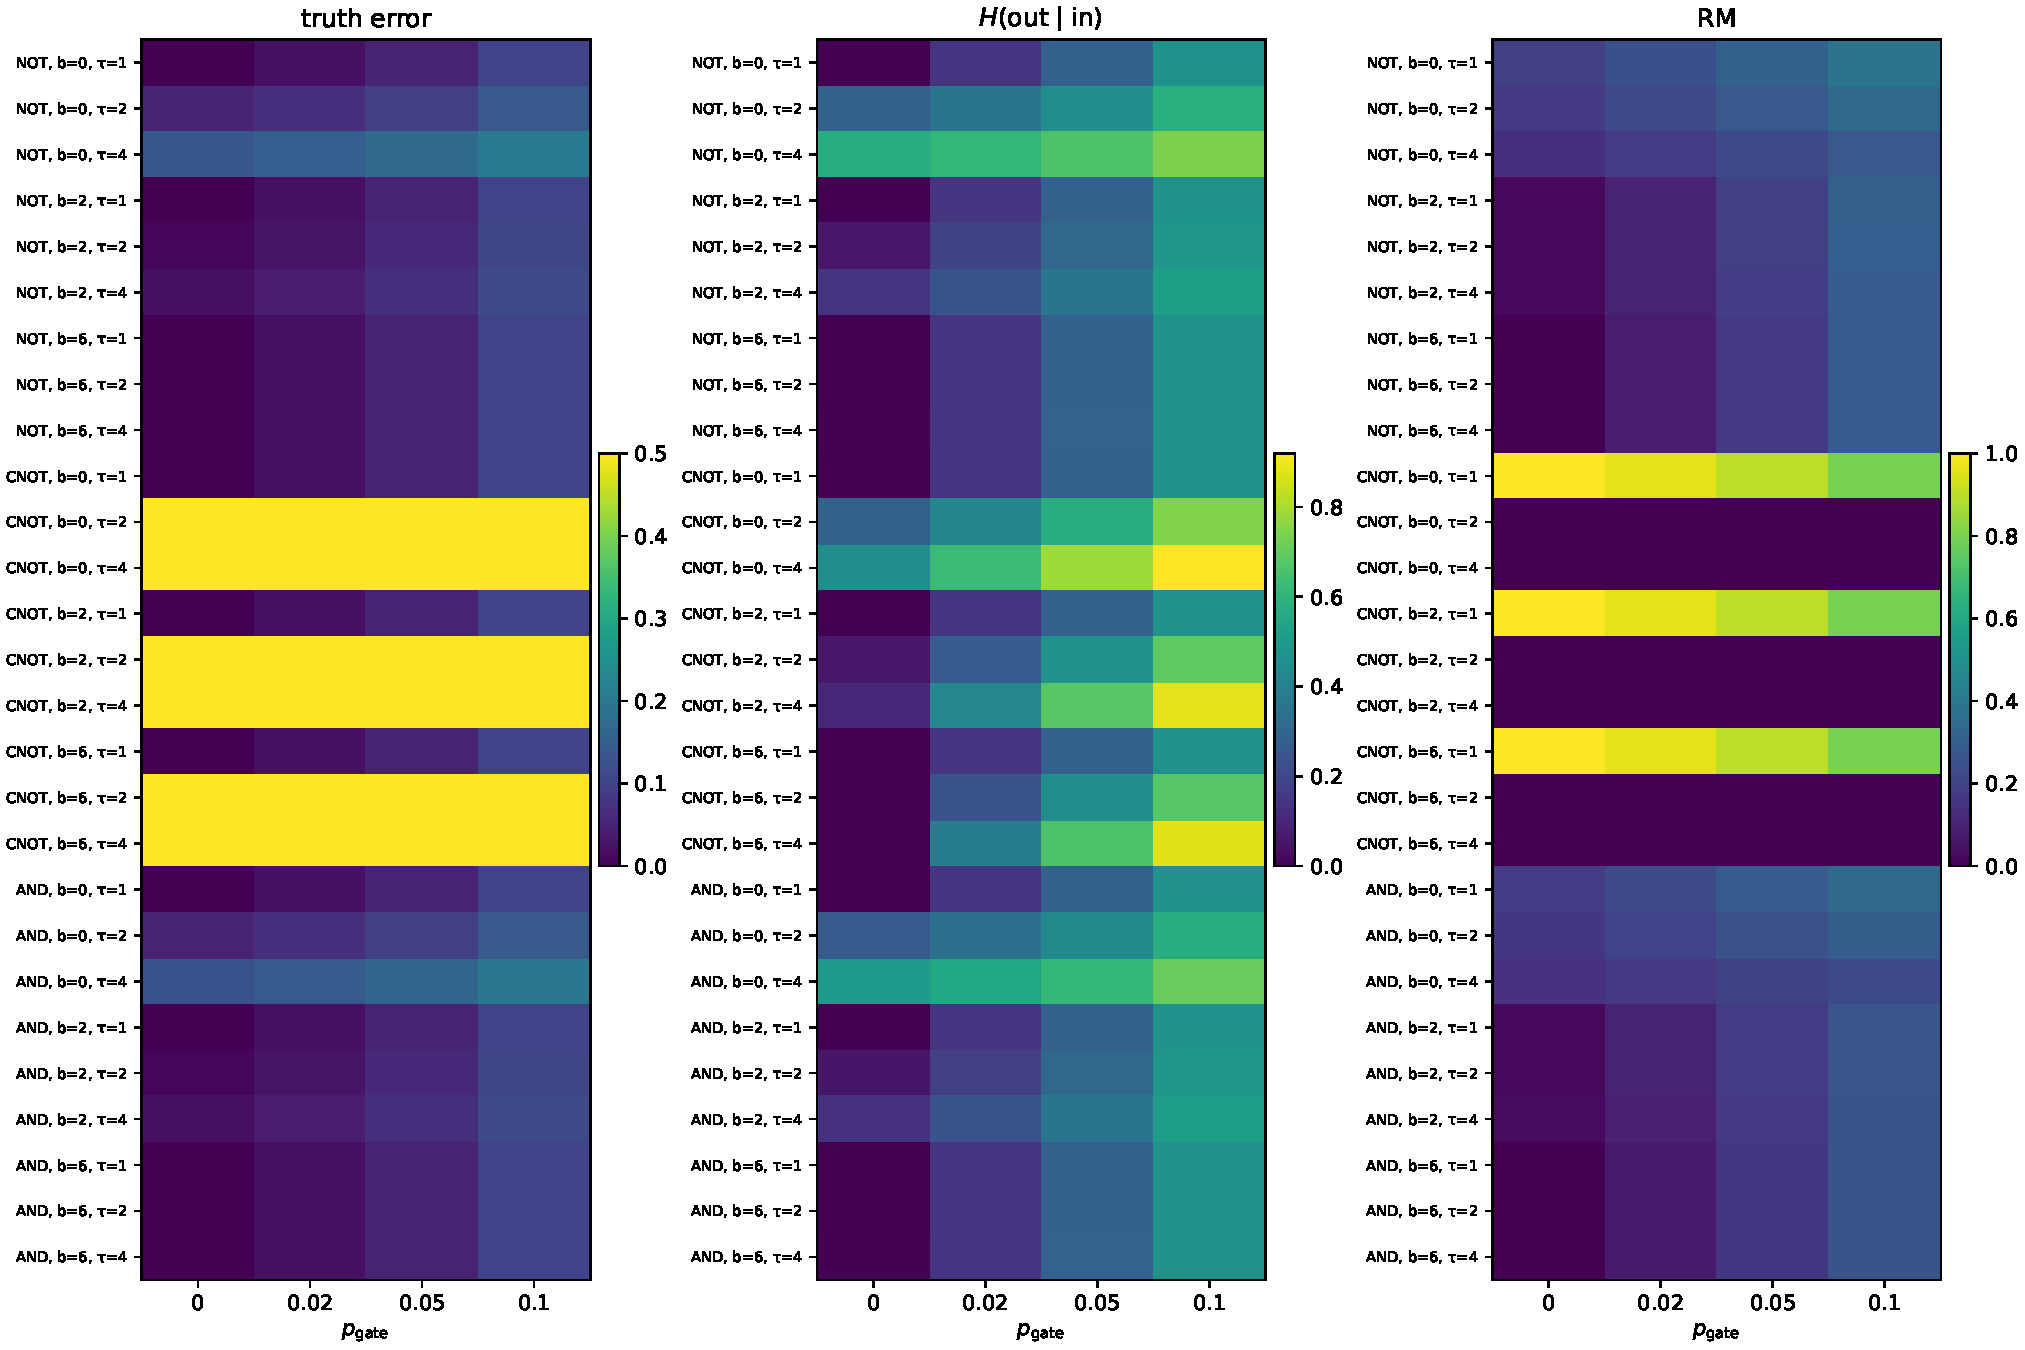
\includegraphics[width=\linewidth]{figures/gate_phase.pdf}
    \caption{Gate-closure phase portrait rendered directly from \protect\path{results/final_claims/figure_gate_phase.csv}. Each row corresponds to a specific gate, barrier, and timescale \(\tau\), while the columns scan output noise \(p_{\mathrm{gate}}\). The three panels report truth error, conditional entropy, and route mismatch on the output-bit lens. The figure is a frozen export of the full \(108\)-row phase bundle.}
    \label{fig:gate-phase}
\end{figure}

At the coarsest level, the frozen bundle shows a clean monotonic trend in truth error with increasing output noise and no anomaly rows. Averaging over barrier and \(\tau\), the NOT truth error rises from \(0.0236\) at \(p_{\mathrm{gate}}=0\) to \(0.1189\) at \(p_{\mathrm{gate}}=0.1\). AND rises from \(0.0225\) to \(0.1180\). CNOT rises from \(0.3333\) to \(0.3667\). These averages are useful as a synopsis, but Figure~\ref{fig:gate-phase} also makes clear why averages alone are insufficient: barrier and horizon matter almost as much as gate noise, and the three diagnostics do not move together in the same way for all gates.

For NOT and AND, the intended gate is recovered cleanly when staging is strong and the evaluation window is short. At barrier \(6\), \(\tau=1\), and \(p_{\mathrm{gate}}=0\), both gates are exact at the channel level in the frozen bundle. NOT records \(\mathrm{err}_{\mathrm{truth}}=0\), \(H(\mathrm{out}\mid\mathrm{in})=0\), and \(\mathrm{RM}=0.000496\). AND records \(\mathrm{err}_{\mathrm{truth}}=0\), \(H(\mathrm{out}\mid\mathrm{in})=0\), and \(\mathrm{RM}=0.000496\). Once the horizon is extended under weak staging, however, closure degrades even when output noise is absent because the stable input bits themselves begin to wander. At barrier \(0\), \(\tau=4\), and \(p_{\mathrm{gate}}=0\), NOT rises to error \(0.1355\), entropy \(0.5723\), and RM \(0.1385\); AND rises to error \(0.1263\), entropy \(0.4974\), and RM \(0.1419\). The symbolic form of the gate has not changed, but the regime in which it is being evaluated has: carrier stability and closure have become the limiting factors.

CNOT behaves differently because the plotted closure lens is intentionally incomplete. At \(\tau=1\) and \(p_{\mathrm{gate}}=0\), the one-step reversible XOR embedding is exact as a gate channel: for barrier \(6\), the frozen bundle records \(\mathrm{err}_{\mathrm{truth}}=0\) and \(H(\mathrm{out}\mid\mathrm{in})=0\). But the RM of the output-bit lens is simultaneously maximal, \(\mathrm{RM}=1\). This is not a contradiction. It is evidence that the output bit alone is not a closed state description for CNOT because its future depends on the retained control bit. The reversible two-bit gate is orderly at the full carrier level, while the one-bit output lens by itself is non-Markovian. CNOT therefore separates channel fidelity from closure in a way that NOT and AND do not.

That separation becomes even sharper at longer horizons. For CNOT, the \(\tau>1\) rows are best read as closure stress tests rather than as repeated grading of the same static truth table. A second noiseless CNOT application toggles the target again, so the one-step XOR truth table is no longer the correct target at \(\tau=2\). This is exactly what appears in the frozen bundle. At barrier \(6\), \(\tau=2\), and \(p_{\mathrm{gate}}=0\), the truth error jumps to \(0.5\), yet the induced error is only \(0.000124\), the conditional entropy is \(0.0018\), and the RM collapses to \(5.55\times 10^{-17}\). At \(\tau=4\), the same pattern persists, with truth error \(0.5\), induced error \(0.000248\), entropy \(0.0033\), and RM \(2.22\times 10^{-16}\). The message is not that CNOT ceases to be structured. The message is that the relevant macro-operator has changed with the protocol horizon. Evaluating \(\tau>1\) as a closure stress test rather than as a truth-table scorecard is therefore essential.

The figure as a whole should be read as a phase portrait of embodied logic. Output noise raises channel error in the expected way, but staging barriers and evaluation horizons determine whether that noise is the dominant failure mode or merely one contributor among several. For NOT and AND, the central transition is from a short-horizon, high-barrier regime in which the gate practically closes, to a longer-horizon, weak-staging regime in which memory corruption drives both entropy and mismatch upward. For CNOT, the key lesson is different: closure depends on retaining the right carrier set. A reversible two-bit gate can be channel-perfect at one horizon while its one-bit output lens remains maximally unclosed.

This regime-based reading sets up the accounting comparison in the next section. The phase portrait already suggests that reversible embedding and erased output are not equivalent descriptions of the same logical object. Section~\ref{sec:results-reversible} makes that distinction explicit by comparing the retained CNOT view and the erased XOR view inside the same underlying laboratory.

\section{Reversible Embedding versus Erased XOR}
\label{sec:results-reversible}

Table~\ref{tab:reversible-erased} isolates the accounting point of the paper in its cleanest form. All three rows come from the same underlying CNOT laboratory at the same noise setting. What changes is not the substrate but the package presented to the layer. The micro row keeps the full \(12\)-state laboratory. The retained macro row packages those microstates into the full four logical CNOT macrostates \((a,b)\). The XOR-erased row keeps only the one-bit output lens and forgets the retained control bit. In Six Birds terms, the split happens at P5: retaining or discarding side information changes the carrier of the layer. P6 then records the consequences.

\begin{table}[t]
    \centering
    \caption{Three views of the same CNOT laboratory: the full microstate view, the retained four-state CNOT macro view, and the XOR-erased one-bit output view. The table reports closure defect, route mismatch, entropy-production rate, and channel-information quantities, showing how forgetting the retained control bit changes both closure and retained information. Rendered directly from \protect\path{results/final_claims/table_reversible_vs_erased.csv}.}
    \label{tab:reversible-erased}
    {\small
\setlength{\tabcolsep}{4pt}
\renewcommand{\arraystretch}{1.12}
\begin{tabularx}{\linewidth}{@{}>{\raggedright\arraybackslash}X r r r r@{}}
\toprule
\multicolumn{5}{@{}l}{\textit{Closure and audit metrics}} \\
\midrule
{View} & {States} & {Defect} & {RM} & {EPR} \\
\midrule
CNOT micro & 12 & 0 & 0 & \(2.72\times 10^{-17}\) \\
CNOT macro & 4 & \(3.47\times 10^{-18}\) & \(1.70\times 10^{-16}\) & 0 \\
XOR erased macro & 2 & 0.96 & 0.96 & 0 \\
\bottomrule
\end{tabularx}

\medskip

\begin{tabularx}{\linewidth}{@{}>{\raggedright\arraybackslash}X r r r r r r@{}}
\toprule
\multicolumn{7}{@{}l}{\textit{Channel-information metrics}} \\
\midrule
{View} & {$H_{\mathrm{in}}$} & {$H_{\mathrm{out}}$} & {\makecell{$H(\mathrm{out}\mid$\\$\mathrm{in})$}} & {\makecell{$I(\mathrm{in};$\\$\mathrm{out})$}} & {$\Delta H$} & {$U_{\text{loss}}$} \\
\midrule
CNOT micro & 2 & 2 & 0.141 & 1.859 & 0 & 0.141 \\
CNOT macro & 2 & 2 & 0.141 & 1.859 & 0 & 0.141 \\
XOR erased macro & 2 & 1 & 0.141 & 0.859 & 1 & 1.141 \\
\bottomrule
\end{tabularx}
}

\end{table}

The first comparison to notice is that the micro and retained macro views are effectively the same logical object at different levels of description. The micro view has closure defect \(0\), RM \(0\), and a numerically tiny entropy-production rate \(2.72\times 10^{-17}\). The retained macro view has closure defect \(3.47\times 10^{-18}\), RM \(1.70\times 10^{-16}\), and apparent EPR \(0\). More importantly, their channel information measures agree at the logical level: both have \(H_{\mathrm{in}}=2\), \(H_{\mathrm{out}}=2\), \(H(\mathrm{out}\mid\mathrm{in})=0.141\), \(I(\mathrm{in};\mathrm{out})=1.859\), and \(U_{\text{loss}}=0.141\). The retained macro row is therefore not an information-poor shadow of the micro description. It is the same reversible embedding expressed at the carrier level that actually closes.

The erased XOR row is qualitatively different. Once the retained control bit is forgotten, the closure defect jumps to \(0.96\) and the RM jumps to \(0.96\). The frozen claims bundle records these as deltas of \(0.96\) and \(0.96\) relative to the retained macro view. At the same time, the channel information profile changes from a two-bit reversible embedding to a many-to-one reported output: \(H_{\mathrm{out}}\) drops from \(2\) to \(1\), \(I(\mathrm{in};\mathrm{out})\) drops from \(1.859\) to \(0.859\), and \(U_{\text{loss}}\) rises from \(0.141\) to \(1.141\). The resulting ratio of unretained input information is \(8.07\). This is the main accounting result of the section.

Two features of Table~\ref{tab:reversible-erased} are especially instructive. First, the conditional entropy \(H(\mathrm{out}\mid\mathrm{in})\) remains \(0.141\) in all three rows. The local noise on the reported output bit has not changed. What changes is how much of the input structure the reported channel can still carry once the control bit is forgotten. This is why the correct comparison is not simply entropy drop but unretained input information. Second, the apparent EPR of the two macro views is \(0\) in both cases. The decisive audit signal here is therefore not a large coarse thermodynamic signature; it is the joint change in closure and retained information. Forgetting side information does not merely add a surcharge to the same logical object. It produces a different logical object.

That distinction is the core P5/P6 lesson. Packaging is not an innocent matter of notation. The retained macro row keeps the full reversible carrier and therefore supports a closed two-bit operator. The erased XOR row reports only a one-bit summary and thereby turns a reversible embedding into a many-to-one channel with large closure failure. What looks superficially like ``the same XOR gate viewed more coarsely'' is, at the level of the audited layer, a different object with different closure properties and a much larger loss ledger.

The point matters beyond this one example. Many discussions of physical logic treat reversible and irreversible descriptions as though the latter were simply the former with some bookkeeping omitted. Table~\ref{tab:reversible-erased} shows why that is too weak. Omitting the bookkeeping changes the closure status of the layer itself. The next section turns from this comparison of declared views to the inverse problem: whether stable packaged bits and a gate can be recovered directly from transition structure without declaring the relevant logical objects in advance (Section~\ref{sec:results-discovery}).

\section{Discovering Bits and Gates}
\label{sec:results-discovery}

The final empirical step reverses the usual implementation story. Up to this point the paper has taken candidate packaged bits and gate lenses seriously enough to ask whether they close. Here we ask whether those bits and a gate can be recovered from transition structure without naming them in advance. The discovery pipeline does not begin with declared symbols such as ``input bit,'' ``parity,'' or ``NOT.'' It begins with the kernel itself: binary partitions are proposed from spectral structure, scored by metastability minus route mismatch, and only then interpreted as candidate packaged predicates. In the NOT reconstruction, candidate output partitions are ranked by future information gain over present redundancy so that a good output bit predicts the future without merely restating the current input partition. Tables~\ref{tab:partition-discovery} and \ref{tab:gate-discovery} report the frozen outputs of that procedure.

\begin{table}[tbp]
    \centering
    \caption{Unsupervised binary partition recovery in the NOT and parity-sector laboratories. The table reports agreement with the intended packaged predicate, candidate-set size, and the top three closure scores. Rendered directly from \protect\path{results/final_claims/table_partition_discovery.csv}.}
    \label{tab:partition-discovery}
    {\footnotesize
\setlength{\tabcolsep}{3.5pt}
\renewcommand{\arraystretch}{1.12}
\begin{tabular*}{\linewidth}{@{\extracolsep{\fill}} l r r r r r r r}
\toprule
{Lab} & {Agree.} & {Cand.} & {Score} & {Meta.} & {RM} & {2nd} & {3rd} \\
\midrule
NOT & 1 & 5 & 1.000 & 1.000 & \(5.55\times 10^{-17}\) & 0.990 & 0.970 \\
Parity sector & 1 & 5 & 0.950 & 0.950 & \(1.70\times 10^{-16}\) & 0.723 & 0.606 \\
\bottomrule
\end{tabular*}
}

\end{table}

Table~\ref{tab:partition-discovery} shows that unsupervised partition recovery succeeds exactly in both benchmark laboratories. In the NOT laboratory, the best recovered partition matches the packaged bit with agreement \(1\) over a candidate set of size \(5\). Its winning score is \(1.000\), with metastability \(1.000\) and RM \(5.55\times 10^{-17}\). The second and third candidate scores, \(0.990\) and \(0.970\), show that the laboratory contains nearby closure-friendly cuts, but the top-ranked partition is the exact packaged distinction. In the parity-sector laboratory, the best recovered partition also has agreement \(1\) with \(5\) candidates considered. Its winning score is \(0.95\), with RM \(1.70\times 10^{-16}\), while the second and third scores fall to \(0.723\) and \(0.606\). The inverse problem is therefore nontrivial but decisive: from transition structure alone, the intended packaged bits emerge as the top-ranked closure variables.

\begin{table}[tbp]
    \centering
    \caption{Recovered NOT gate from discovered input and output partitions. The table reports the fitted truth table, fitted error, fitted entropy, sample size, and the discovery scores used to rank the recovered carriers. Rendered directly from \protect\path{results/final_claims/table_gate_discovery.csv}.}
    \label{tab:gate-discovery}
    {\small
\setlength{\tabcolsep}{5pt}
\renewcommand{\arraystretch}{1.12}
\begin{tabularx}{\linewidth}{@{}l X l X@{}}
\toprule
Metric & Value & Metric & Value \\
\midrule
Gate & NOT & Truth bits & \texttt{[1,0]} \\
Truth table & \texttt{[0,1,1,0]} & Error & 0.0485 \\
Entropy & 0.280 & Sample size & 20000 \\
Input score & 1.000 & $\Delta I_{\mathrm{out}}$ & 0.714 \\
$I_{\mathrm{future}}$ & 0.714 & $I_{\mathrm{current}}$ & 0 \\
\bottomrule
\end{tabularx}
}

\end{table}

Once the input partition has been found, the NOT reconstruction asks a harder question: which binary partition of behavioral classes is the right output bit? Table~\ref{tab:gate-discovery} records the winning answer. The recovered input partition enters the final gate fit with score \(1.000\). The selected output partition has \(\Delta I_{\mathrm{out}}=0.714\), \(I_{\mathrm{future}}=0.714\), and \(I_{\mathrm{current}}=0\). In other words, the chosen output bit carries future information while not merely duplicating the current input partition. On a balanced sample of 20000 transitions, the induced gate fit yields truth bits \texttt{[1,0]}, equivalently the flattened one-step table \texttt{[0,1,1,0]}. That is precisely the NOT gate. The fitted error is \(0.0485\) and the conditional entropy is \(0.280\). The recovery is therefore not a symbolic relabeling of hand-specified registers; it is an induced operator found only after the carriers on which it closes have themselves been discovered.

Taken together, Tables~\ref{tab:partition-discovery} and \ref{tab:gate-discovery} close the empirical arc of the paper. Earlier sections argued that logic should be diagnosed by stability, closure, and audit rather than assumed from symbolic convenience. The discovery results show that the same diagnostics can also work in reverse: they can first detect which packaged distinctions a substrate supports and then recover the operator induced on them. In that sense, the paper does not merely reinterpret known bits and gates inside the Six Birds vocabulary. It shows that a logic layer can be found from dynamics alone. Section~\ref{sec:discussion} returns to the broader implication: logic is something a layer earns, not something an analyst is entitled to assume.

\section{Discussion}
\label{sec:discussion}

This paper began with a prior question to the usual implementation story: when does a substrate actually earn a logic layer? The answer developed through Definition~\ref{def:logic-layer} and the results of Sections~\ref{sec:results-parity}--\ref{sec:results-discovery} is intentionally stricter than being able to label states by \(0\) and \(1\). A logic layer requires packaged predicates that persist, induced operators that close on those predicates, and an audit that measures mismatch and loss. In that sense, logic is not primitive. It is earned by closure.

The first empirical lesson is that parity specialness should be read as a measurement, not a mysticism. Figure~\ref{fig:parity-robustness} showed that, in the parity-sector laboratory, the parity lens beats the median random binary partition at every one of the \(12\) tested grid points, for a win rate of \(1.0\). The point of that result is not that XOR occupies a privileged metaphysical tier. It is that parity is the packaged distinction most naturally aligned with the sector structure of that laboratory. A substrate can therefore make some logical forms cheap and robust without making all familiar Boolean predicates equally natural. The title of the paper is meant in exactly that empirical sense: to ``XOR a stone'' is to discover that parity can be the first logical distinction a substrate stabilizes.

The second lesson is that gate closure is a regime phenomenon rather than a binary yes/no verdict. Figure~\ref{fig:gate-phase} showed that NOT and AND close cleanly in short-horizon, high-barrier regimes and degrade under longer horizons and weaker staging, even when output noise is absent. CNOT revealed a different kind of nonclosure: a one-step reversible XOR embedding can be channel-perfect while the one-bit output lens remains maximally unclosed. This is why the paper has treated \(\tau>1\) CNOT rows as closure stress tests rather than as repeated scoring of the same static truth table. Different gates fail in different ways because closure depends not only on noise but also on the carrier set retained by the layer.

The third lesson is that forgetting side information can change the logical object itself. Table~\ref{tab:reversible-erased} did not compare two unrelated systems; it compared three views of the same CNOT laboratory. The retained macro view and the erased XOR view differ in closure defect by \(0.96\), in route mismatch by \(0.96\), and in unretained input information by a factor of \(8.07\). That is not adequately described as ``the same gate with a larger thermodynamic bill.'' It is a change in what counts as the state of the layer. In Six Birds terms, P5 and P6 are inseparable here: packaging determines the carrier, and the audit reveals that discarding the retained control bit converts a reversible two-bit operator into a many-to-one one-bit report with radically different closure properties \cite{bennett1982thermodynamics,parrondo2015thermoinfo,esposito2012coarsegraining,kawaguchi2013hiddenepr}.

The fourth lesson is that the framework is operational in both directions. Tables~\ref{tab:partition-discovery} and \ref{tab:gate-discovery} showed that the same diagnostics used to test closure can also be used to discover it. The best recovered partitions in the NOT and parity laboratories both achieved agreement \(1.0\), and the recovered NOT gate had truth table \texttt{[0,1,1,0]} with fitted error \(0.04845\). Those results matter because the pipeline begins from transition structure, not from declared symbolic variables. The framework is therefore not merely a reinterpretation of gates we already knew were present. It provides a way to ask, from dynamics alone, which packaged distinctions deserve logical status and which induced operators actually live on them.

Several limitations define the scope of the present paper. First, the laboratories are finite controlled Markov systems chosen for diagnostic clarity rather than for direct substrate realism. Second, the discovery pipeline is restricted to binary partitions and simple gate recovery; it does not yet search higher-arity packages or richer operator vocabularies. Third, the paper is not a full survey of nonclassical logic. It does not attempt to classify all possible failures of complement, negation, or distributivity under coarse-graining.
For partition-based routes from classical state spaces to complementary observables and non-Boolean propositional structures, see \cite{ellerman2010partitions,atmanspacher2015nonboolean}; for the canonical quantum-logical background, see \cite{birkhoff1936quantumlogic}; for a Six Birds programmatic extension in that direction, see \cite{tsiokos2026quantum}.
Those omissions are deliberate. They keep the central claim narrow, falsifiable, and testable: logic layers are measurable closures, not explanatory defaults.

The broader consequence is a pluralistic one. The question is not whether logic is ``really there'' behind every coarse description. The question is which closures a layer can stably support, at what horizon, and with what audit cost. A layer may support parity while failing conjunction, may support a reversible operator only on a larger carrier, or may admit packaged predicates without a low-cost global complement. The Six Birds viewpoint does not eliminate the diversity of logics; it explains that diversity by tying each logic to the closures a substrate can actually sustain.

If there is a final conclusion to draw from XOR, it is not that parity is magical. It is that substrates tell us which distinctions deserve logical status. Logic is not what a theorist can name at a layer, but what a substrate can stabilize, close, and audit there.

\appendix
\section{Reproducibility, frozen artifacts, and formal support}
\label{sec:appendix}

This appendix records the support structure behind the main text and nothing more. The goal is to make the paper reproducible without turning the appendix into a second results section. The main manuscript reads only frozen outputs; no scientific quantity is recomputed during drafting.

\subsection{Reproducibility and artifact manifest}
The repository contains an end-to-end reproduction harness that regenerates the experimental outputs used in the manuscript. The command \texttt{make reproduce-all} rebuilds the six result families used in the paper: the parity-versus-AND sweep, the parity-robustness experiment, the gate-phase bundle, the reversible-versus-erased comparison, the discovery smoke run, and the NOT gate-discovery run. The resulting files are recorded in \path{results/final_manifest.json}, which stores relative paths, file hashes, and sizes for the generated artifacts. This manifest is the repository-level answer to the question ``what exact files underwrite the paper?''

\subsection{Frozen claims bundle}
The manuscript-level interface to those artifacts is the frozen claims bundle under \path{results/final_claims/}. The file \path{claims.json} stores the headline scalar values cited in the paper, while the CSV files store the figure-ready and table-ready data used to render the parity figure, the phase figure, the reversible-versus-erased comparison table, the partition-discovery summary, and the gate-discovery summary. The paper is written against this bundle rather than against live computations. This is why the numerical claims in Sections~\ref{sec:results-parity}--\ref{sec:results-discovery} can be checked line by line against a fixed artifact set.

\subsection{Code and data availability}
All code used to generate the laboratories, diagnostics, discovery pipeline, frozen claims, and paper assets is contained in the public repository at \url{https://github.com/ioannist/six-birds-logic}. Core implementations live under \path{src/emergent_logic/}. Experiment entrypoints live under \path{experiments/}, configuration files under \path{configs/}, and reproducibility / validation utilities under \path{scripts/}. Rendered paper assets are generated from \path{results/final_claims/} by \path{scripts/render_paper_assets.py}. No external proprietary dataset is required for the results reported here. The Lean formalization supporting the definability and quotient-dynamics claims lives under \path{lean/LogicClosure/}.

\subsection{Overflow metric notes}
For compactness, the main text reports only the diagnostics needed to support the paper's central claims. The full frozen phase bundle, however, retains the complete \(108\)-row grid of gate, barrier, horizon, and output-noise conditions in \path{results/final_claims/figure_gate_phase.csv}. Likewise, the parity-robustness asset preserves the full \(12\)-point grid over leakage and horizon in \path{results/final_claims/figure_parity_robustness.csv}. Throughout the repository and manuscript, Shannon quantities such as conditional entropy, mutual information, and unretained input information are reported in bits, whereas entropy-production rates are reported in nats per step.

\section{Brief note on the Lean formalization}
\label{sec:appendix-lean}

The Lean development is intentionally small and local to the paper's logical core. It formalizes three claims. First, definable predicates---those constant on the fibers of a lens---are closed under conjunction, disjunction, and negation. Second, if a micro-update respects an equivalence relation, then it induces a well-defined map on the corresponding quotient. Third, these quotient-dynamics ideas can be instantiated in a concrete finite example: a parity lens from \(\mathrm{Fin}\ 4\) to \(\mathrm{Fin}\ 2\) together with a parity-respecting update. The formalization is not intended as a mechanized version of the full experimental pipeline. Its role is narrower: it certifies the quotient-and-definability skeleton on which the paper's notion of a logic layer rests.

\bibliographystyle{unsrtnat}
\bibliography{refs}


\end{document}
